\section{仿真实验}\label{sec:experiments}
\subsection{场景、比较方法与评价设置}\label{sec:baselines}
四站坐标分别为$(500,0)$、$(0,500)$、$(-500,0)$和$(0,-500)$\,m。以最大站间距离定义基线$R=\max_{l,v}\|\bm r_l-\bm r_v\|_2=1000$\,m。搜索区域为$[-1000,1000]^2$\,m$^2$，真实源位置为连续坐标，不要求落在初始网格上。两源采用独立BPSK符号，经根升余弦（RRC）脉冲成形；符号率$R_s=10$\,MHz、滚降系数$\alpha_{\mathrm{RRC}}=0.25$，对应名义带宽$B=(1+\alpha_{\mathrm{RRC}})R_s=12.5$\,MHz。表\ref{tab:scenario}汇总公共设置。

\begin{table}[H]\centering\small
\caption{公共仿真参数。}\label{tab:scenario}
\begin{tabularx}{.96\linewidth}{@{}lX@{}}\toprule
参数 & 设置\\\midrule
接收站／源数 & 四个同步单天线站；已知$K=2$\\
传播 & 自由空间相对幅度$1/d$与基带时延；$c_0=299792458$\,m/s\\
波形 & 独立BPSK；RRC成形，符号率10\,MHz，滚降0.25\\
中心与名义带宽 & 两源中心均为0；带宽均为12.5\,MHz\\
采样与记录 & 50\,MHz；8192点；163.84\,$\mu$s\\
处理频带 & $[-7,7]$\,MHz；完整记录DFT保留2293个频点\\
噪声与信噪比 & 时域复噪声方差1；源B四站平均带内SNR为6\,dB\\
平均接收功率差 & 0、3、6、9、12、15\,dB；固定源B与噪声，仅缩放源A\\
初始网格 & 各方法统一20\,m，$101\times101=10201$点\\
候选间距 & 30\,m；AP联合版本分别保留1、2、5个候选\\
正式规模 & 20布局$\times$20随机实现$\times$6档功率差，共2400条\\
共同子集 & 各布局预先固定2次实现，保留全部功率差，共240条\\\bottomrule
\end{tabularx}
\end{table}

两源的符号、波形初相和定时独立。同一布局与随机实现的六档功率差共用波形和噪声，因而可以直接观察另一源增强带来的变化。源A为功率扫描源，源B为固定源；在正功率差下分别称强源和弱源，0\,dB时采用A／B标记。各方法只处理预先指定的公共频带$[-7,7]$\,MHz，在名义带宽两侧各留0.75\,MHz保护带，不提供逐源波形或频谱。筛选频点不重新缩放DFT，也不作逐站混合功率归一化。

正式比较采用20个布局，覆盖双源均在站内、A外B内、A内B外和双源均在站外四类构型，每类5个。站内指四站凸包内部，站外仍位于搜索区域内。几何生成排除距任一站小于150\,m、距中心小于100\,m、距站点对连线小于50\,m的位置，两源间距至少300\,m。位置按预定几何约束生成，不按定位结果筛选。图\ref{fig:formalgeometry}展示全部布局。

实验先在共同240条观测上比较八类方法，再将核心方法的随机重复从每布局2次增加到20次，形成2400条扩展验证。两组均覆盖全部20布局和六档功率差，区别在于随机重复次数；240条是2400条的预先固定子集，不额外增加样本总数。全面比较用于衡量各方法的可靠性与成本，扩展验证则用于检查核心方法的表现及收益来源。
\begin{figure}[htbp]\centering
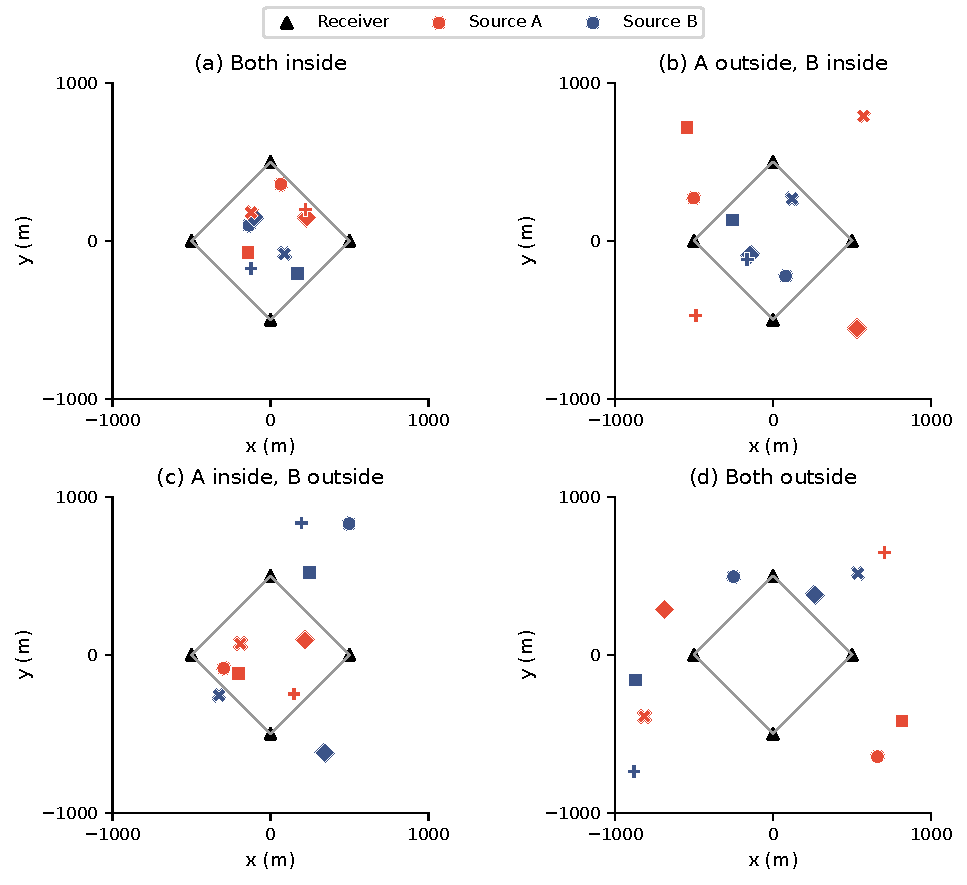
\includegraphics[width=.88\linewidth]{figures/formal_geometry.pdf}
\caption{20个源站布局，每类5个。黑色三角形为接收站，灰色菱形边界为站点凸包；同一面板内，相同形状的两个标记为一对源，红色为源A、蓝色为源B。0\,dB时两源平均接收功率相同。}\label{fig:formalgeometry}
\end{figure}
\FloatBarrier
图\ref{fig:formalgeometry}覆盖站内与站外的四类组合，使方法比较同时包含不同的源站位置关系。同一面板用五种形状区分五对源，颜色只区分源A与源B；各功率条件保持对应位置不变。

所有方法共享IQ观测、已知传播信息、搜索区域和20\,m初始网格，保留各自的连续精修。LS谱、MUSIC、MVDR、AP、块NOMP、SBL、多初值联合ML和GA联合ML的本场景准则列于附录\ref{app:baselines}；具体参数见表\ref{tab:parameters}。多初值ML采用去重的谱峰组合与Sobol空间覆盖起点，GA采用128个体，避免因重复初始化削弱搜索覆盖。MUSIC以同一记录的四个片段估计协方差，按扣除噪声后的观测功率加权；MVDR-known使用八个片段，相对对角加载为0.01。两者均只分析公共处理带内的频点，不将MVDR-known称为原版DPD-HR。
\par\begin{table}[H]\centering\footnotesize
\caption{正式比较采用的方法参数。连续位置优化不受20\,m网格量化。}\label{tab:parameters}
\begin{tabularx}{\linewidth}{@{}p{.18\linewidth}p{.27\linewidth}X@{}}\toprule
版本 & 核心操作 & 参数\\\midrule
LS谱 & 单源LS谱取两个峰 & 共同20 m网格；同谱连续精修\\
MUSIC & 噪声子空间宽带汇聚 & 4段；超噪声功率加权；已知K\\
MVDR-known & 加载协方差逆谱 & 8段；相对加载0.01\\
充分AP & 反复全域条件更新 & 候选5；循环上限6；正常连续精修\\
交替／联合AP & 相同分支，改变精修方式 & 候选1/2/5；每次局部上限100；共同投影梯度阈值$10^{-8}$\\
VP-BNOMP & 残差发现、消元Newton、共同LS & 循环上限10000；能量变化阈值$10^{-8}$；每次Newton最多5步；步长上限50 m；局部小步阈值0.01 m\\
固定系数BNOMP & 原文对应的固定系数更新 & 循环上限10000；能量阈值$10^{-8}$；局部小步阈值0.01 m\\
多初值联合ML & 同一联合LS目标 & 8个唯一初值：4谱峰+4 Sobol；L-BFGS-B\\
GA联合ML & 同一联合LS目标 & 种群128；最多200代；连续30代停滞停止\\
宽带SBL & 共享功率、离网字典、单点$\gamma$ & 最多300轮；每5轮离网更新；8个活动点；原生停止\\
\bottomrule\end{tabularx}\end{table}
\par
表\ref{tab:parameters}区分每种方法的搜索、精修和停止设置。各方法共享初始网格，但不强求相同迭代次数；AP按共同梯度精度比较，固定系数与消元块NOMP则保留相同原生循环停止规则。
运行环境为Windows、Python 3.10.20、NumPy 2.2.6和PyTorch 2.8.0+cu129，GPU为NVIDIA GeForce RTX 4070 Ti SUPER，CPU计算线程设为20。响应与目标使用双精度实数／复数运算。
\par

\FloatBarrier
\paragraph{定位评价}
设真实与估计集合分别为$X=\{\bm p_k\}$、$Y=\{\widehat{\bm p}_j\}$。容许误差预先设为基线的2\%，即$r=0.02R=20$\,m，与初始网格步长分别定义。成功评价在距离不超过$r$的关联中先最大化一对一匹配数，再最小化平方距离和；双源成功要求两源同时匹配，单个估计不能重复对应两个真源。位置误差则使用最小平方距离指派\cite{Kuhn1955}：
\begin{equation}
 \pi^*=\arg\min_{\pi}\sum_{k=1}^{K}\|\bm p_k-\widehat{\bm p}_{\pi(k)}\|_2^2,
 \qquad e_{ik}=\|\bm p_{ik}-\widehat{\bm p}_{i,\pi^*(k)}\|_2 .\label{eq:assignment}
\end{equation}
其中$i$为观测编号，$k$为源编号，$\pi$为估计编号的排列，$e_{ik}$单位为m。对$n$条观测，RMSE和经验累计分布函数（CDF）为
\begin{equation}
 \operatorname{RMSE}_k=\sqrt{\frac1n\sum_{i=1}^{n}e_{ik}^2},\qquad
 \widehat F_k(t)=\frac1n\sum_{i=1}^{n}\mathbf 1(e_{ik}\le t).\label{eq:rmseCDF}
\end{equation}
式中$\mathbf 1$为示性函数，P95为误差的第95百分位数。RMSE和CDF使用全部样本，包括未达到成功门槛的样本。GOSPA\cite{Rahmathullah2017}保留为辅助集合指标，取$p=2$、$c=100$\,m、$\alpha=2$，其定义为
\begin{equation}
 d_{\mathrm G}(X,Y)^2=\min_{\gamma}\left[
 \sum_{(k,j)\in\gamma}\|\bm p_k-\widehat{\bm p}_j\|^2
 +\frac{c^2}{2}\left(|X|+|Y|-2|\gamma|\right)\right].\label{eq:gospa}
\end{equation}
这里$\gamma$为一对一部分关联，$|\cdot|$表示集合基数。正文以成功率、RMSE、CDF和耗时为主要比较依据。

\paragraph{成本与统计}
完整算法时间包含IQ输入后的DFT、频带筛选、传输、搜索、系数重估和精修，GPU计时同步，公共预热单列。在线轨迹记录计入登记墙钟，磁盘持久化及事后精度证书不计入求解时间；各方法独立承担搜索与初始化成本。目标、梯度、响应及循环调用分别统计，包含梯度计算的目标请求不与梯度次数相加。布局内同一实现的六档功率差保持配对；不确定性按构型类别、布局及随机实现分层重采样。核心比较和共同子集比较分别统计。

\subsection{八类方法的共同观测比较}\label{sec:commonformal}
首先比较各类方法在相同混合观测上的恢复能力与完整计算成本。表\ref{tab:formalcommon}使用各布局两次固定实现及全部六档功率差，共240条，所有方法逐条配对。VP-BNOMP采用同批运行的消元实现，各方法成本均来自这组共同观测。
\begin{table}[H]\centering\small
\caption{同一240条观测上的基线与提出方法比较。成功门槛20\,m；RMSE和P95单位为m，时间单位为s。}\label{tab:formalcommon}
\begin{tabular}{@{}lrrrrrr@{}}\toprule
方法 & 双源成功 & 成功率/\% & 强源RMSE & 弱源RMSE & 弱源P95 & 时间\\\midrule
LS谱取峰 & 38/240 & 15.83 & 191.982 & 845.184 & 1708.755 & 0.2368\\
宽带MUSIC & 151/240 & 62.92 & 93.515 & 646.892 & 1701.876 & 0.2015\\
MVDR-known & 75/240 & 31.25 & 320.684 & 804.082 & 1706.625 & 0.1925\\
充分AP & 240/240 & 100.00 & 0.876 & 1.596 & 4.229 & 8.9076\\
固定系数BNOMP & 228/240 & 95.00 & 0.906 & 89.706 & 30.998 & 2.9416\\
VP-BNOMP & 228/240 & 95.00 & 0.875 & 86.177 & 18.913 & 0.5907\\
多初值联合ML & 45/240 & 18.75 & 256.061 & 776.935 & 1719.566 & 1.2227\\
GA联合ML & 185/240 & 77.08 & 279.056 & 501.231 & 1634.174 & 8.0702\\
宽带SBL & 240/240 & 100.00 & 1.096 & 3.743 & 8.962 & 44.1296\\
五候选联合AP & 240/240 & 100.00 & 0.876 & 1.596 & 4.229 & 0.7081\\
\bottomrule\end{tabular}\end{table}

在相同观测上，MCJ-AP以更低成本达到了充分AP和SBL的恢复水平。三者均全部成功，平均完整耗时分别为0.708\,s、8.908\,s和44.130\,s。固定系数BNOMP与VP-BNOMP均成功228条；消元版本的平均耗时由2.942\,s降至0.591\,s。两者保留相同发现和循环后共同LS结构，局部系数处理的差别在第\ref{sec:mechanismresults}节分析。
\begin{figure}[htbp]\centering
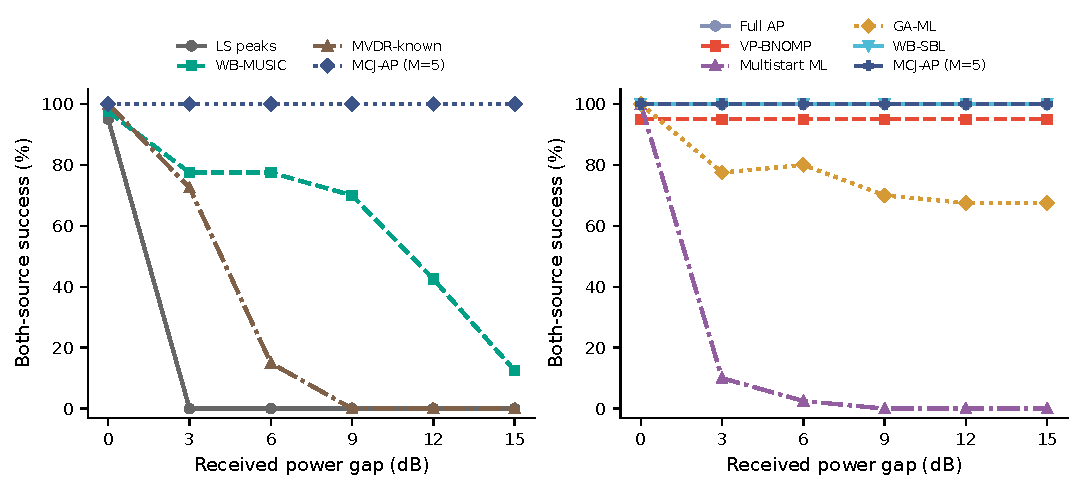
\includegraphics[width=\linewidth]{figures/formal_common.pdf}
\caption{共同240条观测的功率差扫描，每档40条。左侧比较谱方法，右侧比较逐源与联合求解方法；两个面板使用同一五候选AP参照。}\label{fig:formalcommon}
\end{figure}
\FloatBarrier

\begin{samepage}
图\ref{fig:formalcommon}显示，MUSIC与MVDR-known在功率差增大后明显退化，整体成功率分别为62.92\%和31.25\%；LS谱取峰为15.83\%。逐源或联合拟合能够更好地处理本组混合观测。多初值ML成功率为18.75\%，充分AP则达到100\%；二者使用同一联合目标，结果差别体现了初始化与搜索路径的重要性。GA成功率为77.08\%，平均耗时为8.070\,s。
\end{samepage}

MCJ-AP兼顾高恢复率与较低计算成本，VP-BNOMP则以较少计算取得95\%的双源成功率。SBL有226条按原生稳定条件停止、14条达到300轮上限。辅助GOSPA、耗时P95与共同子集停止状态见表\ref{tab:auxiliary}。

\FloatBarrier
\subsection{核心方法的2400条扩展验证}\label{sec:coreformal}
增加随机重复后，MCJ-AP仍保持较高的恢复率，VP-BNOMP保持较低的逐源更新成本。表\ref{tab:formalcore}汇总全部20布局、2400条观测；VP-BNOMP采用第\ref{sec:vpnomp}节的消元Newton实现。
\begin{table}[H]\centering\small
\caption{全部2400条观测的核心比较。成功门槛20\,m；RMSE和P95单位为m，时间单位为s。}\label{tab:formalcore}
\begin{tabular}{@{}lrrrrrr@{}}\toprule
方法 & 双源成功 & 成功率/\% & 强源RMSE & 弱源RMSE & 弱源P95 & 时间\\\midrule
单候选联合AP & 2280/2400 & 95.00 & 0.897 & 107.265 & 25.194 & 0.3958\\
双候选联合AP & 2280/2400 & 95.00 & 0.897 & 103.698 & 25.194 & 0.4704\\
五候选联合AP & 2376/2400 & 99.00 & 0.896 & 46.984 & 3.845 & 0.7180\\
VP-BNOMP & 2278/2400 & 94.92 & 0.892 & 74.193 & 217.599 & 0.5855\\
\bottomrule\end{tabular}\end{table}

五候选MCJ-AP成功2376条，将单候选的95\%成功率提高至99\%，平均耗时为0.718\,s。两者的强源RMSE均约0.897\,m，弱源恢复没有降低强源精度。VP-BNOMP成功2278条，成功率为94.92\%，平均耗时0.586\,s。该版本由单独完成的同输入验证计时，严格的消元更新效率比较采用第\ref{sec:mechanismresults}节的同批共同观测。

功率差既可能影响正确区域内的定位精度，也可能改变候选选择。图\ref{fig:formalcore}将本批诊断发现的布局4与其余19布局分开，分别观察这两种影响。两组均保留全部随机实现、功率条件和失败结果，总体成绩见表\ref{tab:formalcore}。
\begin{figure}[htbp]\centering
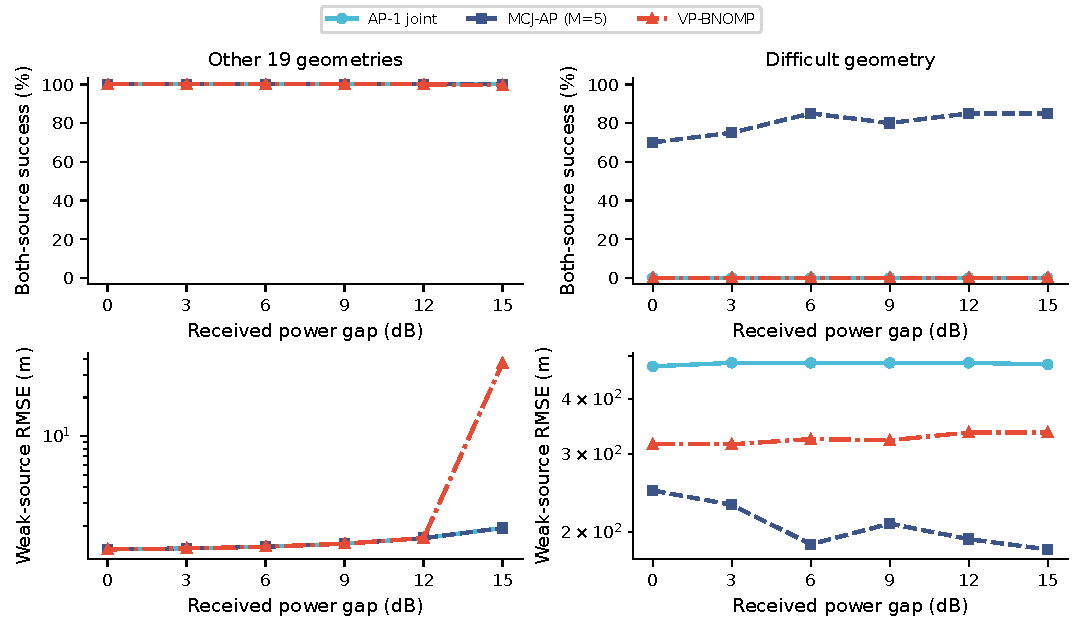
\includegraphics[width=.94\linewidth]{figures/formal_core.pdf}
\caption{扩展验证中功率差的分组结果。左列为其余19布局，共2280条、每档380条；右列为困难布局4，共120条、每档20条。上行为双源成功率，下行为弱源RMSE。分组依据本批构型诊断，全部2400条仍计入总体统计。}\label{fig:formalcore}
\end{figure}
\FloatBarrier
其余19布局中，两种AP均全部成功，MCJ-AP的弱源RMSE随功率差从1.31\,m增至1.93\,m，显示强源增强后弱源定位精度逐步下降。VP-BNOMP在这一组有两条15\,dB失败，因此该档RMSE仍受到长尾影响。右列单独呈现候选恢复困难，具体失败分布和候选机制在第\ref{sec:timecases}节集中分析。

\begin{figure}[htbp]\centering
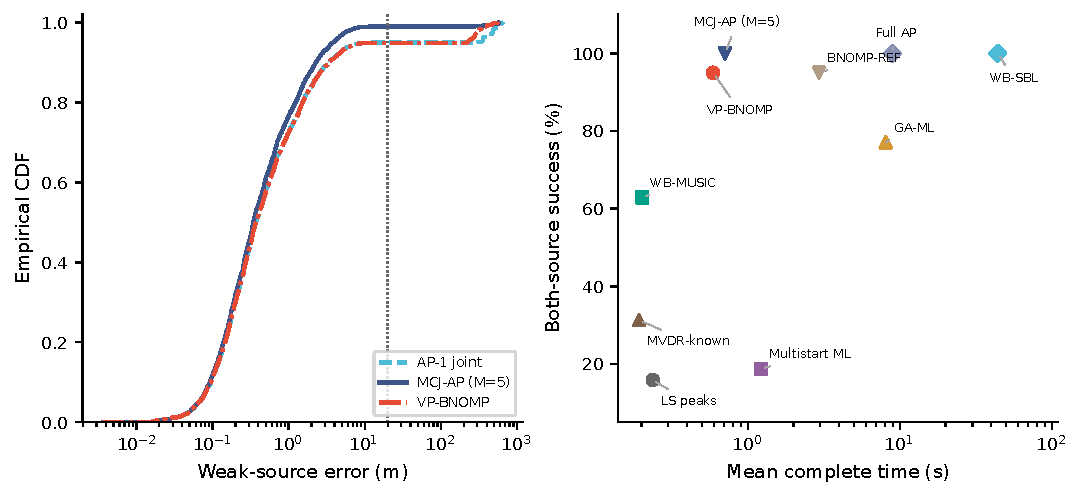
\includegraphics[width=\linewidth]{figures/formal_cdf_cost.pdf}
\caption{误差分布与可靠性--成本取舍。左：全部2400条核心观测的弱源CDF，虚线标出20\,m；右：同一240条共同子集的双源成功率与平均完整耗时。两个面板的样本范围分别标明，不跨样本范围排名。}\label{fig:formalcdfcost}
\end{figure}
\FloatBarrier
图\ref{fig:formalcdfcost}左图使用全部2400条观测，补充展示总体误差分布。MCJ-AP的弱源P95为3.85\,m、RMSE为46.98\,m，大多数结果准确，少量远距离错误拉高了RMSE。右图回到第\ref{sec:commonformal}节的共同240条比较成本：VP-BNOMP具有较低的计算开销，MCJ-AP则以额外候选处理换取更高恢复率。两个面板分别回答误差分布和同输入成本问题。

\FloatBarrier
\subsection{候选保留提高可靠性，联合精修减少计算}\label{sec:apresults}
图\ref{fig:formalablation}将候选保留与联合精修的作用分别展示，避免把增加候选带来的额外成本与精修本身的节省混在一起。
\begin{figure}[htbp]\centering
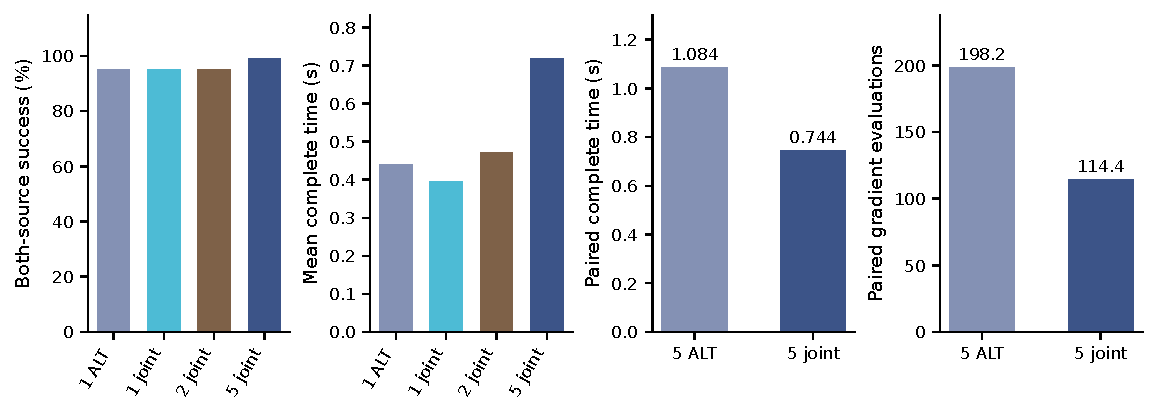
\includegraphics[width=\linewidth]{figures/formal_ablation.pdf}
\caption{AP的候选与精修消融，四面板单行排列。左两图为原2400条主批的成功率与耗时，右两图为同一2400条输入上的五候选配对耗时与梯度计算。ALT为交替精修，joint为联合精修；左、右两批分别计时，不跨批计算加速比。}\label{fig:formalablation}
\end{figure}
\FloatBarrier
左两图显示，候选数为1和2的联合AP均成功2280条，五候选增至2376条。第二候选尚未覆盖本批困难区域，保留更多有效起点才带来恢复。右两图显示，在候选数相同的条件下，联合精修同时减少实际耗时和梯度计算。

单候选配对先说明了联合精修的省时作用：相同成功数和接近的RMSE下，平均耗时从0.439\,s降至0.396\,s，减少9.84\%。平均耗时差（联合减交替）的95\%分层配对区间为$[-0.0496,-0.0367]$\,s；目标计算从39.76次降至28.69次，梯度计算从37.76次降至26.69次。

为确认省时不是降低求解精度造成的，表\ref{tab:fivepair}单独列出五候选配对的精度和尾部指标。两种版本对每条观测使用相同的五个初始候选，在同一完整目标和投影梯度阈值下停止；运行顺序交错，共2400对、4800次求解。
\begin{table}[H]\centering\small
\caption{相同五候选配对的定位精度，2400对；计算成本见图\ref{fig:formalablation}。}\label{tab:fivepair}
\begin{tabular}{@{}lrrrrr@{}}\toprule
精修方式 & 双源成功 & 强源RMSE/m & 弱源RMSE/m & 弱源P95/m & GOSPA/m\\\midrule
交替 & 2376 & 0.896 & 46.983 & 3.846 & 2.099\\
联合 & 2376 & 0.896 & 46.984 & 3.845 & 2.100\\
\bottomrule\end{tabular}\end{table}

表\ref{tab:fivepair}中，两者均成功2376条，成功／失败身份逐例一致；强源RMSE约0.896\,m，弱源P95约3.85\,m，弱源RMSE和GOSPA也几乎相同。这说明联合更新保留了交替更新的定位质量，效率改善并非以更早放弃困难样本为代价。与表中精度结果对应，图\ref{fig:formalablation}右两图显示平均完整耗时从1.0840\,s降至0.7441\,s，减少31.36\%；耗时差的95\%分层配对区间为$[-0.3691,-0.3121]$\,s。

省时与计算量减少一致：平均联合目标计算从204.21次降至120.36次，梯度计算从198.21次降至114.36次，后者减少约42.30\%。两种版本选中分支均满足共同梯度条件，全部候选中有两次交替精修触及安全迭代上限，其结果仍计入统计。由此，多候选保留了困难弱源的有效起点，联合精修则以更少局部计算处理这些候选，两者共同构成MCJ-AP的可靠性与效率收益。

\FloatBarrier
\subsection{波形消元更新的机制与效率}\label{sec:mechanismresults}
式\eqref{eq:schur}给出了固定系数与消元曲率之间的关系。位置改变时，波形系数可以补偿一部分响应变化，固定系数曲率没有扣除这部分耦合，可能产生反复的小步。局部消元同时改变更新方向和试探位置的目标计算，因此应与保留相同外层时序的参照配对，区分局部更新收益与整套实现差别。

在同批共同240条上，固定系数与消元版本都成功228条，平均完整耗时分别为2.9416\,s和0.5907\,s，消元版本减少约79.92\%的计算时间，见表\ref{tab:formalcommon}。这一对照保持残差发现、逐源循环和循环后共同LS的时序，局部更新将固定系数Newton及其回溯目标改为式\eqref{eq:localprofile}的消元形式。结合式\eqref{eq:schur}，它直接检验了位置--波形耦合处理对计算效率的作用。

在全部2400条上，VP-BNOMP与早期NOMP的成功集合逐例一致，保持了相同的恢复能力，整体精度与成本见表\ref{tab:formalcore}。二者共同成功观测中的VP-BNOMP弱源RMSE约1.52\,m；这一条件统计用于观察已恢复位置的精度，总体评价仍包含全部失败。与MCJ-AP相比，VP-BNOMP侧重减少逐源更新成本，多候选AP侧重扩大有效候选覆盖。

VP-BNOMP全部观测均按相邻循环的归一化残差能量变化不超过$10^{-8}$停止，平均记录约51.03轮，没有达到10000轮安全上限。该上限仅防止异常长循环，不代表实际需要接近此数量的迭代。每次局部Newton最多5步，位置试探上限50\,m，接受小步小于0.01\,m时结束本次局部调用。推导、伪代码、参数表及上述统计均对应同一消元实现。

\subsection{求解时间轨迹与困难构型的候选恢复}\label{sec:timecases}
图\ref{fig:formaltime}重放共同240条观测上已经保存的输出。尚无双源输出的观测按未成功计；RMSE仅在全部观测有输出后显示。
\begin{figure}[htbp]\centering
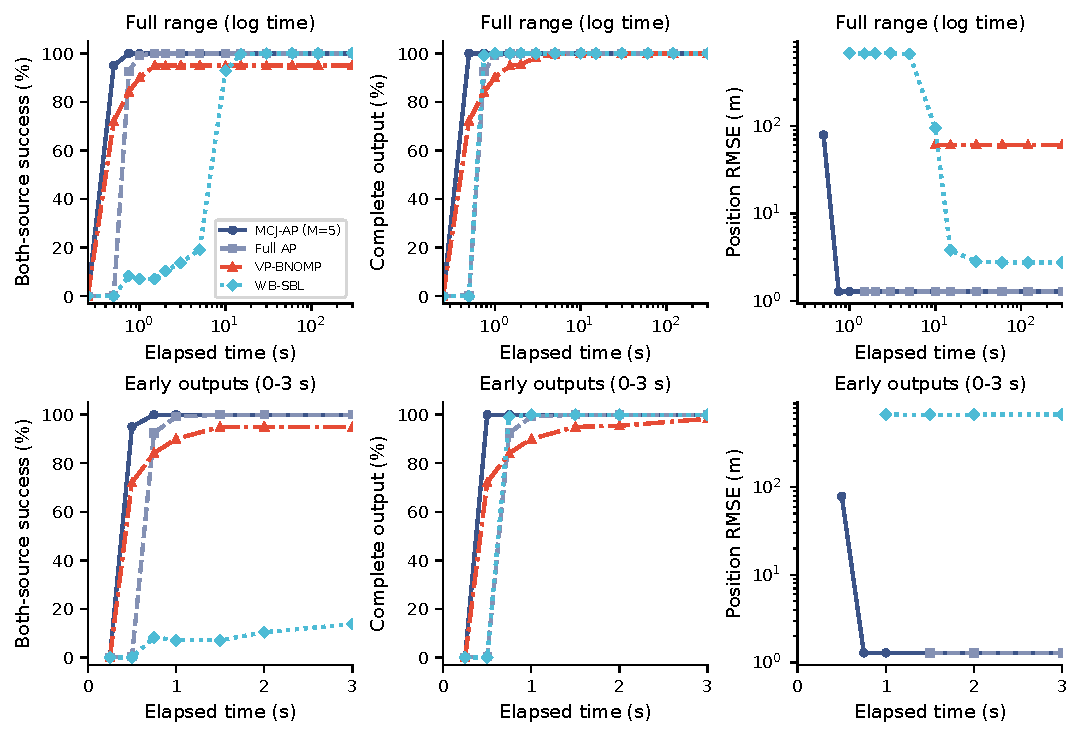
\includegraphics[width=\linewidth]{figures/formal_time.pdf}
\caption{共同240条观测的保存输出轨迹。上行使用0.25--300\,s对数时间轴，下行以线性时间轴放大0--3\,s；三列依次为双源成功率、完整输出比例和位置RMSE。正常停止后保持最终值，RMSE纵轴仍用对数刻度。连接线表示保存点之间的变化，不额外规定算法停止时刻。}\label{fig:formaltime}
\end{figure}
\FloatBarrier

五候选联合AP在0.75\,s保存点达到全部成功，充分AP在2\,s达到相同成功数，SBL在30\,s达到相同成功数。因此，取得高质量结果的时间与完成全部计算的时间需要分别观察。上行对数轴便于比较亚秒至数百秒的差异，下行则分辨早期输出。VP-BNOMP在本次登记轨迹中只发布最终完整双源结果，其曲线不代表内部每次循环均已有对外输出。

\paragraph{困难构型下的候选覆盖}
图\ref{fig:formallayouts}给出全部20布局的失败分布，用于定位总体长尾的来源。
\begin{figure}[htbp]\centering
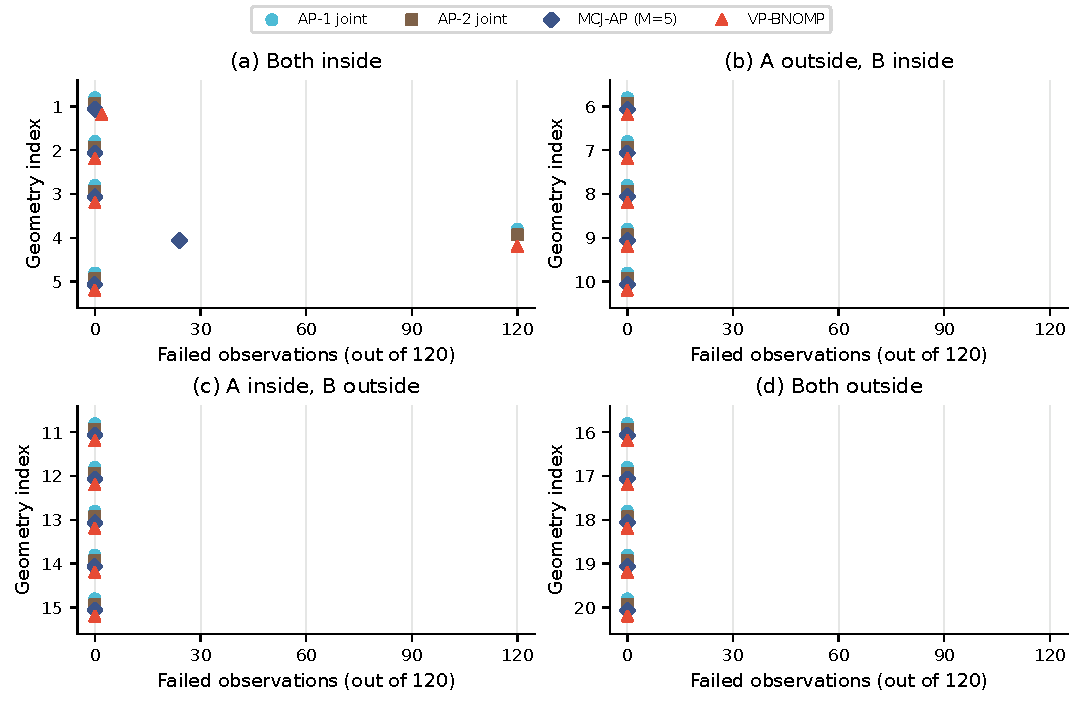
\includegraphics[width=\linewidth]{figures/formal_layouts.pdf}
\caption{各布局的双源失败数，每布局120条。四个面板对应四类构型，零表示该布局全部成功；不同标记在纵向稍作错开，便于辨认重合结果。}\label{fig:formallayouts}
\end{figure}
\FloatBarrier
单候选AP在布局4的120条观测上全部失败，五候选恢复其中96条，其余19布局没有成功转失败。VP-BNOMP在布局4全部失败，另外两条失败位于其余布局的15\,dB条件。多候选的可靠性收益因而集中在本批困难构型，下面通过候选位置和精修目标解释这一恢复过程。

MCJ-AP每档400条观测中有3--6条失败，均来自布局4，并贡献各档超过99.7\%的弱源平方误差。该布局内候选选择的变化主导了总体RMSE折线的非单调起伏；其余19布局的曲线则更清楚地显示功率差对定位精度的影响。同一组布局在六档功率差中保持不变，这种起伏并非各档采用了不同构型。

图\ref{fig:formalcandidates}给出同一困难布局的恢复与未恢复案例，以对照候选覆盖和最终选择。
\begin{figure}[htbp]\centering
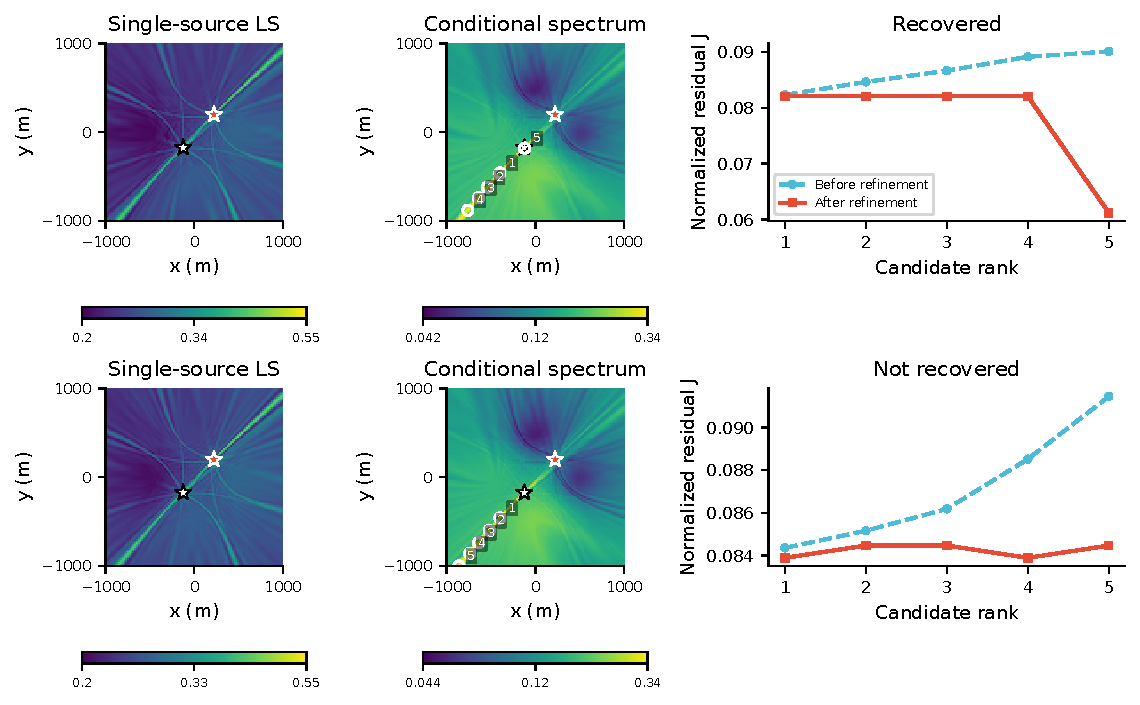
\includegraphics[width=\linewidth]{figures/formal_candidates.pdf}
\caption{同一困难构型的两个0\,dB事后机制案例。左列为单源LS谱，中列为条件谱，右列为候选精修前后残差；上行为恢复案例，下行为未恢复案例。红色和白色星号分别标示源A、源B，空心圆为条件候选。谱图采用对数色标，右列连接线仅连接候选编号，不表示实际迭代路径。}\label{fig:formalcandidates}
\end{figure}
\FloatBarrier
上行中，前四个候选都进入远端错误区域，第五候选则接近真实源B。联合精修后，第五分支得到更低残差，源B误差约0.09\,m。下行的五个候选均落在远端高分带，最近起点仍距源B约397\,m，局部精修未能恢复。这表明粗谱最高分与精修后的最佳位置并不等价；多候选增加有效起点，最终拟合负责择优，两者共同提高恢复能力。若候选全部落在错误区域，局部精修本身不能补足全域覆盖。

第\ref{sec:complexity}节的复杂度分析与实际调用量相对应：单／五候选AP均只作两次全域网格扫描，增加分支主要增加连续目标和梯度计算；固定系数与消元NOMP则需比较局部导数调用和循环成本。这些计数用于解释候选覆盖与局部更新各自带来的开销和收益。
